\documentclass{article}
\usepackage[utf8]{inputenc}

\title{Week 8 Lecture 1}
\author{Jared Brannan }

\usepackage{natbib}
\usepackage{graphicx}
\graphicspath{ {./figures/} }
\usepackage{mathtools}
\usepackage{amsthm}
\usepackage{amsmath}
\usepackage{amssymb}
\usepackage{xcolor}
\usepackage{bbm}
\usepackage{bm}
\usepackage{physics}

% indent first line
\usepackage{indentfirst}
% one inch margins
\usepackage[margin=1.0in]{geometry}

\theoremstyle{definition}

\newcommand{\upRiemannint}[2]{
\overline{\int_{#1}^{#2}}
}
\newcommand{\loRiemannint}[2]{
\underline{\int_{#1}^{#2}}
}

\newtheorem{definition}{Definition}
\newtheorem{asside}{Asside}
\newtheorem{conjecture}{Conjecture}
\newtheorem{example}{Example}
\newtheorem{theorem}{Theorem}
\newtheorem{lemma}{Lemma}
\newtheorem{puzzle}{Puzzle}
\newtheorem{corollary}{Corollary}
\newtheorem{proposition}{Proposition}


\begin{document}
\maketitle

\section{Administrative drivel}
\begin{itemize}
	\item
\end{itemize}

\section{Anatomy and Physiology}

\subsection{Cardiovascular system continued...}
\subsection{Blood vessels}
\begin{itemize}
	\item Blood pressure is usually lower in veins than arteries
	\item veins have check valves to prevent the blood from moving backward
		\begin{itemize}
			\item Helpful in moving blood through the circulatory system
			\item every time you move, the muscles get wider, squeezing the blood vessels, but the blood can't go backward's to make room of this compression due to the valves, so the blood has to resume it's journey to the heart
		\end{itemize}

	\item \textbf{Capillaries} 
		\begin{itemize}
			\item Picks up blood from the arterials, through the tissues, and thenn to the veinules
			\item Smallest blood vessls -- typically 1 blood-cell wide
			\item important because virtually all exchanges between tissue and blood happen in the capilaries
			\item capilaries have very thin walls (1 cell thick, with gaps) allowing things out (and in through diffusion)
			\item \textbf{Capillary bed}  == interwoven net of capillaries entwined throughout \textit{all}  tissue.
			\item this means the body can control which tissues get more/less blood.
			\item Capillary flow is regulated by : smooth muscle cells, \textit{precapillary sphincters}, wrapped around the small arteries prior to capillary beds can contract or relax, under unconscious nervous control
				(each instance is 1 muscle cell)
				\begin{itemize}
					\item open == vasodialation
					\item closed == vasoconstriction
				\end{itemize}
			\item there is a thorough-fare channel (which is itself a capillary) that bipasses the blood past a capilary bed when vasoconstriction occurs.
			\item Adjustable capillaries are found in nearly all tissues
			\item Not all capillary beds are active at the same time 
				\begin{itemize}
					\item Turned up/down by precapillary sphincters
				\end{itemize}
			\item Vasoconstriction/dialation is used for body temperature regulation
				\begin{itemize}
					\item renods desease causes to much vasoconstriction in the hands
					\item After exercise, skin capilary beds open up
				\end{itemize}
		\end{itemize}
	\item closer look at blood vessels:
		\begin{center}
			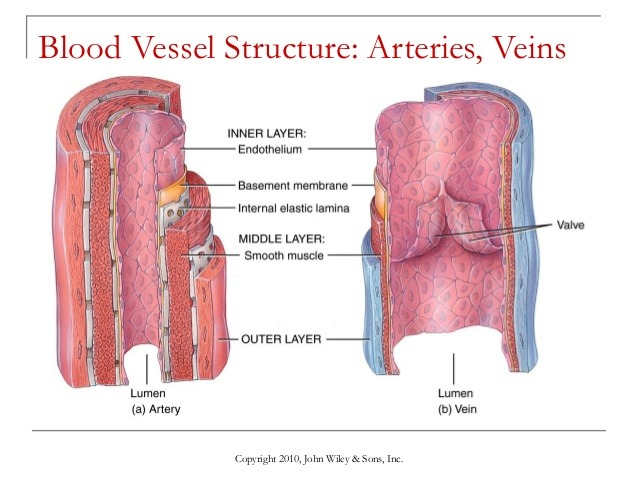
\includegraphics[width=40em]{blood_vessel.jpg}
		\end{center}
	\item Veins are less muscular than arteris, and move the blood much more slowly with very little pressure than the arteries
	\item Veins suffer injury earlier in life since they have a thinner (weaker) structure).
		\begin{itemize}
			\item Valves -- prevent back flow
				\begin{itemize}
					\item Varicose veins==failed valves
					\item Assist in pumping blood
				\end{itemize}
		\end{itemize}
	\item Vessel injuries:
		\begin{itemize}
			\item Capillaries are: low pressure and low volume
				\begin{itemize}
					\item suppose you cut yourself
					\item Slow ooze of little blood 
				\end{itemize}
			\item Veins are: large volume but low pressure
				\begin{itemize}
					\item suppose you cut yourself
					\item Slow ooze of lots of blood 
				\end{itemize}
			\item arteries are: large volume but high pressure
				\begin{itemize}
					\item suppose you cut yourself
					\item Jets of lots of blood the quirts with pulse
					\item these are the most dangerous! won't clot due to high pressure.
				\end{itemize}
		\end{itemize}
	\item clicker q: What kind of muscle do blood vessels have? Smooth
\end{itemize}


\end{document}
